\newpage

\subsection{QuizziPedia::Front-End::Models}

	\label{QuizziPedia::Front-End::Models}
	
	\begin{figure}[ht]
		\centering
		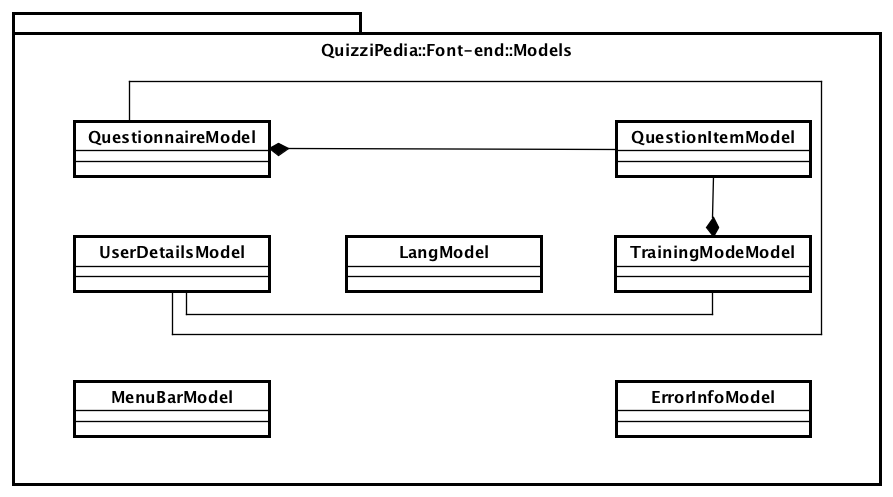
\includegraphics[scale=0.5,keepaspectratio]{UML/Package/QuizziPedia_Front-End_Models.png}
		\caption{QuizziPedia::Front-End::Models}
	\end{figure} \FloatBarrier

	\subsubsection{Informazioni generali}
		\begin{itemize}
			\item \textbf{Descrizione}: package contenente le classi che definiscono la business logic dell'applicazione;
			\item \textbf{Padre}: \texttt{Front-End};
			\item \textbf{Iterazioni con altri componenti}: 
				\begin{itemize}				
					\item \texttt{Controllers}: package contenente i controllers front-end dell'applicazione;
					\item \texttt{Directives}: package contenente le directives front-end dell'applicazione;
					\item \texttt{Models}: package contenente le classi che definiscono la business logic dell'applicazione;
					\item \texttt{Templates}: package contenente i templates necessari per la creazione dinamica delle viste per le domande;
					\item \texttt{Services}: package che contiene le classi individuate che permettono la comunicazione del lato front-end con il lato back-end attraverso l'architettura REST.
				\end{itemize}

		\end{itemize}
	
	\subsubsection{Classi}
		\paragraph{QuizziPedia::Front-End::Models::ErrorInfoModel}
		
		\label{QuizziPedia::Front-End::Models::ErrorInfoModel}
		
		\begin{figure}[ht]
			\centering
			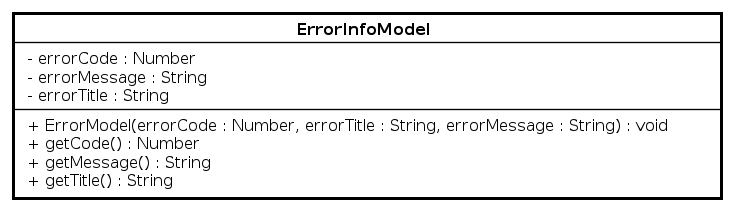
\includegraphics[scale=0.5,keepaspectratio]{UML/Classi/Front-End/QuizziPedia_Front-end_Models_ErrorInfoModel.png}
			\caption{QuizziPedia::Front-End::Models::ErrorInfoModel}
		\end{figure} \FloatBarrier
		
		\begin{itemize}
			\item \textbf{Descrizione}: rappresenta le informazioni di un errore che si è verificato eseguendo una determinata operazione;
			\item \textbf{Utilizzo}: viene utilizzata rappresentare un oggetto di tipo errore;
			\item \textbf{Relazioni con altre classi}: 
			\begin{itemize}
			 	\item \textit{OUT} \texttt{AuthService}: questa classe permette di gestire la registrazione e l'autenticazione di un utente;
			 	\item \textit{OUT} \texttt{SearchService}: questa classe permette di gestire il recupero dei dati dal back-end a seguito di una ricerca effettuata da un utente;
			 	\item \textit{OUT} \texttt{LangService}: questa classe permette di gestire la lingua nella quale si è scelto di utilizzare l'applicazione.
			 	\item \textit{OUT} \texttt{QuizService}: questa classe permette di ottenere i dati di un quiz tramite delle parole chiave inserite dall'utente nella barra di ricerca. Permette inoltre di iscriversi ad un questionario e di scaricare l'intera l'ista di domande di un questionario a partire dal suo id univoco;
			 	\item \textit{OUT} \texttt{StatisticsService}: questa classe permette di ottenere le statistiche dell'utente;
		 		\item \textit{OUT} \texttt{QuestionsService}: questa classe permette di ottenere domande esistenti e salvare nuove domande;
	 			\item \textit{OUT} \texttt{UserDetailsService}: questa classe permette di ottenere i dati personali degli utenti;
			\end{itemize}
			\item \textbf{Attributi}: 
			\begin{itemize}
				\item \texttt{- errorCode: Number} \\ 
				Rappresenta il codice dell'errore;
				\item \texttt{- errorMessage: String} \\ 
				Rappresenta la descrizione dell'errore; 
				\item \texttt{- errorTitle: String}\\ 
				Rappresenta il titolo del messaggio d'errore.
			\end{itemize}
			\item \textbf{Metodi}
			\begin{itemize}
				\item \texttt{+ ErrorModel(errorCode: Number, errorTitle: String, errorMessage: String) : void} \\
				Metodo costruttore della classe.\\
				\textbf{Parametri}: 
				\begin{itemize}
					\item \texttt{errorCode: Number} \\
					Parametro contenente il codice di errore;
					\item \texttt{errorTitle: String} \\
					Parametro contenente il titolo di errore;
					\item \texttt{errorMessage: String} \\
					Parametro contenente il messaggio di errore.
				\end{itemize}
				\item \texttt{+ getCode() : Number} \\
				Metodo che consente di ottenere il codice dell'errore;
				\item \texttt{+ getMessage() : String} \\
				Metodo che consente di ottenere la descrizione dell'errore;
				\item \texttt{+ getTitle() : String} \\
				Metodo che consente di ottenere il titolo del messaggio d'errore. 
			\end{itemize}
		\end{itemize}
			
		\paragraph{QuizziPedia::Front-End::Models::LangModel}
		
		\label{QuizziPedia::Front-End::Models::LangModel}
		
		\begin{figure}[ht]
			\centering
			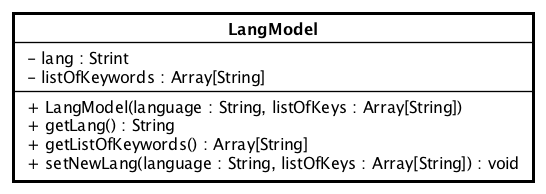
\includegraphics[scale=0.5,keepaspectratio]{UML/Classi/Front-End/QuizziPedia_Front-end_Models_LangModel.png}
			\caption{QuizziPedia::Front-End::Models::LangModel}
		\end{figure} \FloatBarrier
		
		\begin{itemize}
			\item \textbf{Descrizione}: rappresenta le informazioni per la giusta traduzione dell'applicazione;
			\item \textbf{Utilizzo}: viene utilizzata per racchiudere tutte le informazioni riguardanti la giusta traduzione dell'applicazione;
			\item \textbf{Relazioni con altre classi}: 
			\begin{itemize}
				\item \textit{IN} \texttt{LoginController}: questa classe permette di gestire l'autenticazione dell'utente al sistema; 
				\item \textit{IN} \texttt{SignUpController}: questa classe permette di gestire la registrazione di un utente al sistema;
				\item \textit{IN} \texttt{HomeController}: questa classe permette di gestire la home page;
				\item \textit{IN} \texttt{SearchController}: questa classe permette di gestire la ricerca di questionari e utenti all'interno dell'applicazione;
				\item \textit{IN} \texttt{ProfileManagementController}: questa classe permette di gestire il profilo personale di un utente;
				\item \textit{IN} \texttt{LogoutController}: questa classe permette di gestire la pagina di logout;
				\item \textit{IN} \texttt{PasswordForgotController}: questa classe permette di gestire il ripristino della password dimenticata;
				\item \textit{IN} \texttt{TrueFalseQuestionsController}: questa classe permette di gestire la creazione e la modifica di una domanda vero/falso;
				\item \textit{IN} \texttt{MultipleQuestionsController}: questa classe permette di gestire la creazione e la modifica di una domanda a risposta multipla; 
				\item \textit{IN} \texttt{ConnectionQuestionsController}: questa classe permette di gestire la creazione e la modifica di una domanda a collegamento;
				\item \textit{IN} \texttt{ImagesSortingQuestionsController}: questa classe permette di gestire la creazione e la modifica di una domanda a ordinamento immagini;
				\item \textit{IN} \texttt{StringsSortingQuestionsController}: questa classe permette di gestire la creazione e la modifica di una domanda a ordinamento di stringhe;
				\item \textit{IN} \texttt{FillingQuestionsController}: questa classe permette di gestire la creazione e la modifica di una domanda a riempimento di spazi; 
				\item \textit{IN} \texttt{ClickableAreaQuestionsController}: questa classe permette di gestire la creazione e la modifica di una domanda ad area cliccabile;
				\item \textit{IN} \texttt{EditorQMLController}: questa classe permette di gestire la creazione e la modifica di domande create tramite editor QML;
				\item \textit{IN} \texttt{QuestionsManagementController}: questa classe permette di gestire e di ottenere le domande create dall'utente;
				\item \textit{IN} \texttt{TrainingController}: questa classe permette di gestire la modalità allenamento sottoponendo all'utente le giuste domande adatte al suo livello;
				\item \textit{IN} \texttt{FillingQuestionnaireController}: questa classe permette di gestire la compilazione del questionario;
				\item \textit{IN} \texttt{TemplateQuestionnaireController}: questa classe permette di gestire la creazione di un questionario; 
				\item \textit{IN} \texttt{RegistrationManagementController}: questa classe permette di gestire le iscrizione degli utenti ai questionari;
				\item \textit{IN} \texttt{ResultsController}: questa classe permette di gestire i risultati della ricerca effettuata dall'utente;
				\item \textit{IN} \texttt{QuestionnaireManagementController}: questa classe permette di gestire tutti i questionari creati da un utente;  
				\item \textit{IN} \texttt{MenuBarController}: questa classe permette di gestire il menù fisso per ogni pagina;
				\item \textit{IN} \texttt{FooterController}: questa classe permette di gestire il footer dell'applicazione;
				\item \textit{IN} \texttt{ErrorController}: questa classe permette di gestire tutti i messaggi di errore da mostrare all'utente;
			\end{itemize}
			\item \textbf{Attributi}: 
			\begin{itemize}
				\item ;
			\end{itemize}
			\item \textbf{Metodi}: 
			\begin{itemize}
				\item ;
			\end{itemize}
		\end{itemize}
		
		\paragraph{QuizziPedia::Front-End::Models::QuestionItemModel}
		
		\label{QuizziPedia::Front-End::Models::QuestionItemModel}
		
		\begin{figure}[ht]
			\centering
			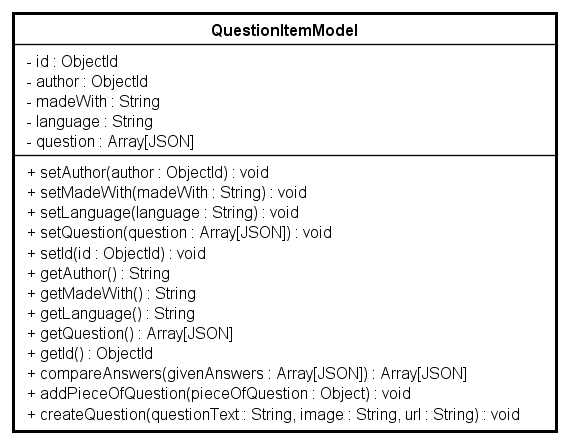
\includegraphics[scale=0.5,keepaspectratio]{UML/Classi/Front-End/QuizziPedia_Front-end_Models_QuestionItemModel.png}
			\caption{QuizziPedia::Front-End::Models::QuestionItemModel}
		\end{figure} \FloatBarrier
		
		\begin{itemize}
			\item \textbf{Descrizione}: rappresenta una domanda. Contiene tutte le informazioni necessarie alla
			presentazione del contenuto della domanda;
			\item \textbf{Utilizzo}: viene utilizzata per memorizzare i dati di una domanda;
			\item \textbf{Relazioni con altre classi}: 
			\begin{itemize}
				\item \textit{IN} \texttt{QuestionsManagementController}: questa classe permette di gestire e di ottenere le domande create dall'utente;
				\item \textit{IN} \texttt{TrueFalseQuestionsController}: questa classe permette di gestire la creazione e la modifica di una domanda vero/falso;
				\item \textit{IN} \texttt{MultipleQuestionsController}: questa classe permette di gestire la creazione e la modifica di una domanda a risposta multipla; 
				\item \textit{IN} \texttt{ConnectionQuestionsController}: questa classe permette di gestire la creazione e la modifica di una domanda a collegamento;
				\item \textit{IN} \texttt{ImagesSortingQuestionsController}: questa classe permette di gestire la creazione e la modifica di una domanda a ordinamento immagini;
				\item \textit{IN} \texttt{StringsSortingQuestionsController}: questa classe permette di gestire la creazione e la modifica di una domanda a ordinamento di stringhe;
				\item \textit{IN} \texttt{FillingQuestionsController}: questa classe permette di gestire la creazione e la modifica di una domanda a riempimento di spazi; 
				\item \textit{IN} \texttt{ClickableAreaQuestionsController}: questa classe permette di gestire la creazione e la modifica di una domanda ad area cliccabile;
				\item \textit{IN} \texttt{EditorQMLController}: questa classe permette di gestire la creazione e la modifica di domande create tramite editor QML;
				\item \textit{IN} \texttt{QuestionsController}: questa classe permette di gestire il recupero delle domande per poterle stampare nella modalità allenamento e nei questionari;
			\end{itemize}
			\item \textbf{Attributi}: 
			\begin{itemize}
				\item ;
			\end{itemize}
			\item \textbf{Metodi}: 
			\begin{itemize}
				\item ;
			\end{itemize}
		\end{itemize}
		
		\paragraph{QuizziPedia::Front-End::Models::QuestionnaireModel}
		
		\label{QuizziPedia::Front-End::Models::QuestionnaireModel}
		
		\begin{figure}[ht]
			\centering
			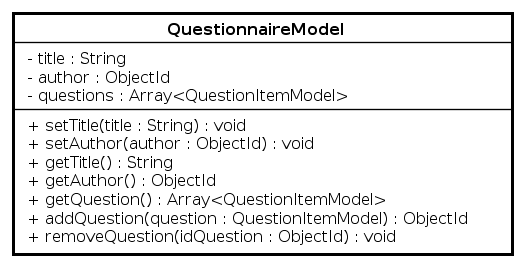
\includegraphics[scale=0.5,keepaspectratio]{UML/Classi/Front-End/QuizziPedia_Front-end_Models_QuestionnaireModel.png}
			\caption{QuizziPedia::Front-End::Models::QuestionnaireModel}
		\end{figure} \FloatBarrier
		
		\begin{itemize}
			\item \textbf{Descrizione}: rappresenta un questionario. Contiene tutte le informazioni necessarie alla
			presentazione del contenuto del questionario;
			\item \textbf{Utilizzo}: viene utilizzata per memorizzare i dati di un questionario;
			\item \textbf{Relazioni con altre classi}: 
			\begin{itemize}
				\item \textit{IN} \texttt{SearchController}: questa classe permette di gestire la ricerca di questionari e utenti all'interno dell'applicazione;
				\item \textit{IN} \texttt{QuestionnaireDetailsController}: questa classe permette di gestire tutti i questionari creati da un utente; 
				\item \textit{IN} \texttt{FillingQuestionnaireController}: questa classe permette di gestire la creazione e la modifica di una domanda a riempimento di spazi;
				\item \textit{IN} \texttt{CreateQuestionnaireController}: questa classe permette di gestire la creazione di un questionario;
				\item \textit{IN} \texttt{RegistrationManagementController}: questa classe permette di gestire le iscrizione degli utenti ai questionari;
				\item \textit{IN} \texttt{ResultsController}: questa classe permette di gestire i risultati della ricerca effettuata dall'utente;
			\end{itemize}
			\item \textbf{Attributi}: 
			\begin{itemize}
				\item ;
			\end{itemize}
			\item \textbf{Metodi}: 
			\begin{itemize}
				\item ;
			\end{itemize}
		\end{itemize}	
		
		\paragraph{QuizziPedia::Front-End::Models::TrainingModeModel}
		
		\label{QuizziPedia::Front-End::Models::TrainingModeModel}
		
		\begin{figure}[ht]
			\centering
			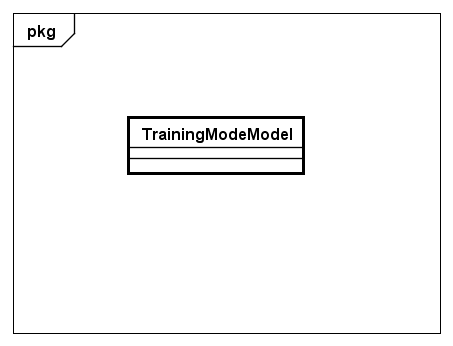
\includegraphics[scale=0.5,keepaspectratio]{UML/Classi/Front-End/QuizziPedia_Front-end_Models_TrainingModeModel.png}
			\caption{QuizziPedia::Front-End::Models::TrainingModeModel}
		\end{figure} \FloatBarrier
		
		\begin{itemize}
			\item \textbf{Descrizione}: rappresenta un allenamento. Contiene tutte le informazioni necessarie alla
			presentazione del contenuto di un allenamento;
			\item \textbf{Utilizzo}: viene utilizzata per memorizzare i dati di un allenamento;
			\item \textbf{Relazioni con altre classi}: 
			\begin{itemize}
				\item \textit{IN} \texttt{TrainingController}: questa classe permette di gestire la modalità allenamento sottoponendo all'utente le giuste domande adatte al suo livello;
			\end{itemize}
			\item \textbf{Attributi}: 
			\begin{itemize}
				\item ;
			\end{itemize}
			\item \textbf{Metodi}: 
			\begin{itemize}
				\item ;
			\end{itemize}
		\end{itemize}
			
		\paragraph{QuizziPedia::Front-End::Models::UserDetailsModel}
		
		\label{QuizziPedia::Front-End::Models:.UserDetailsModel}
		
		\begin{figure}[ht]
			\centering
			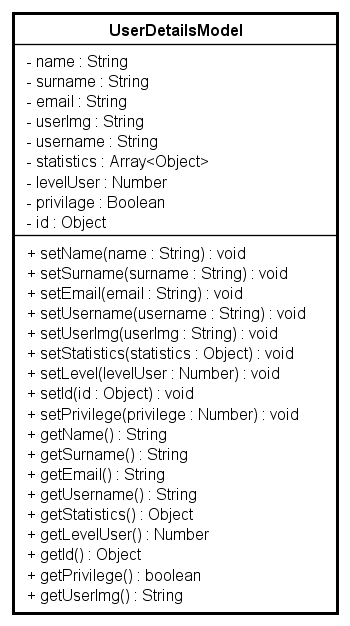
\includegraphics[scale=0.5,keepaspectratio]{UML/Classi/Front-End/QuizziPedia_Front-end_Models_UserDetailsModel.png}
			\caption{QuizziPedia::Front-End::Models::UserDetailsModel}
		\end{figure} \FloatBarrier
		
		\begin{itemize}
			\item \textbf{Descrizione}: rappresenta un utente. Contiene tutte le informazioni necessarie alla
			presentazione del contenuto di un utente sia nella visualizzazione che nella gestione di un profilo;
			\item \textbf{Utilizzo}: viene utilizzata per memorizzare i dati di un utente;
			\item \textbf{Relazioni con altre classi}: 
			\begin{itemize}
				\item \textit{IN} \texttt{LoginController}: questa classe permette di gestire l'autenticazione dell'utente al sistema;
				\item \textit{IN} \texttt{SearchController}: questa classe permette di gestire la ricerca di questionari e utenti all'interno dell'applicazione;
				\item \textit{IN} \texttt{UserDetailsController}: questa classe permette di gestire i dati di un utente;
				\item \textit{IN} \texttt{StatisticsController}: questa classe permette di le statistiche di un utente;
			\end{itemize}
			\item \textbf{Attributi}: 
			\begin{itemize}
				\item ;
			\end{itemize}
			\item \textbf{Metodi}: 
			\begin{itemize}
				\item ;
			\end{itemize}
		\end{itemize}	
		
		\paragraph{QuizziPedia::Front-End::Models::MenuBarModel}
		
		\label{QuizziPedia::Front-End::Models::MenuBarModel}
		
		%\begin{figure}[ht]
		%	\centering
		%	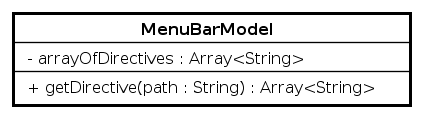
\includegraphics[scale=0.5,keepaspectratio]{UML/Classi/Front-End/QuizziPedia_Front-end_Models_MenuBarModel.png}
		%	\caption{QuizziPedia::Front-End::Models::MenuBarModel}
		%\end{figure} \FloatBarrier
		
		\begin{itemize}
			\item \textbf{Descrizione}: rappresenta un utente. Contiene tutte le informazioni necessarie alla
			presentazione del contenuto di un utente sia nella visualizzazione che nella gestione di un profilo;
			\item \textbf{Utilizzo}: viene utilizzata per memorizzare i dati di un utente;
			\item \textbf{Relazioni con altre classi}: 
			\begin{itemize}
				\item \textit{IN} \texttt{LoginController}: questa classe permette di gestire l'autenticazione dell'utente al sistema;
				\item \textit{IN} \texttt{SearchController}: questa classe permette di gestire la ricerca di questionari e utenti all'interno dell'applicazione;
				\item \textit{IN} \texttt{UserDetailsController}: questa classe permette di gestire i dati di un utente;
				\item \textit{IN} \texttt{StatisticsController}: questa classe permette di le statistiche di un utente;
			\end{itemize}
			\item \textbf{Attributi}: 
			\begin{itemize}
				\item ;
			\end{itemize}
			\item \textbf{Metodi}: 
			\begin{itemize}
				\item ;
			\end{itemize}
		\end{itemize}		
		
		
		\paragraph{QuizziPedia::Front-End::Models::RightDirectiveModel}
		
		\label{QuizziPedia::Front-End::Models::RightDirectiveModel}
		
		%\begin{figure}[ht]
		%	\centering
		%	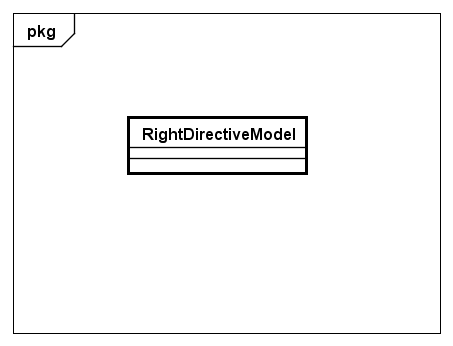
\includegraphics[scale=0.5,keepaspectratio]{UML/Classi/Front-End/QuizziPedia_Front-end_Models_RightDirectiveModel.png}
		%	\caption{QuizziPedia::Front-End::Models::RightDirectiveModel}
		%\end{figure} \FloatBarrier
		
		\begin{itemize}
			\item \textbf{Descrizione}: rappresenta un utente. Contiene tutte le informazioni necessarie alla
			presentazione del contenuto di un utente sia nella visualizzazione che nella gestione di un profilo;
			\item \textbf{Utilizzo}: viene utilizzata per memorizzare i dati di un utente;
			\item \textbf{Relazioni con altre classi}: 
			\begin{itemize}
				\item \textit{IN} \texttt{LoginController}: questa classe permette di gestire l'autenticazione dell'utente al sistema;
				\item \textit{IN} \texttt{SearchController}: questa classe permette di gestire la ricerca di questionari e utenti all'interno dell'applicazione;
				\item \textit{IN} \texttt{UserDetailsController}: questa classe permette di gestire i dati di un utente;
				\item \textit{IN} \texttt{StatisticsController}: questa classe permette di le statistiche di un utente;
			\end{itemize}
			\item \textbf{Attributi}: 
			\begin{itemize}
				\item ;
			\end{itemize}
			\item \textbf{Metodi}: 
			\begin{itemize}
				\item ;
			\end{itemize}
		\end{itemize}														